\chapter{Columnar Compression}
\label{columnar-compression}

Compression in column-oriented storage has been extensively researched \cite{abadi-col-comp, abadi-sparse-col, boncz-comp} in the world of \gls{rdbms}. The main idea of column-specific compression being, 1) the ability to compress each data column independently depending on its datatype and features like runs, sorted etc.; 2) high compression rates since adajcent elements in the column are similar; and 3) with some cases, ability to operate directly on compressed data. However, not all columnar compression techniques can be directly applied to the data-structures that we introduced in Chapter~\ref{c:columnar-storage}. In this chapter, we identify the set of requirements that we want to achieve by compressing our columnar structures. We then review existing compression techniques and propose a technique tha helps us fulfill our reuqirements.

We begin by exploring the set of requirements in Section~\ref{sec:col-existing}. Based on these requirements, we reviewthe applicability of existing columnar compression techniques. Section~\ref{sec:sparse} discusses the case of data sparsity in our columns and why existing solutions to compress spare columns are not applicable. Finally, we end the chapter by introducing a new NULL compression algorithm, \emph{prefixSum-based NULL compression}, that addresses the shortcomings of existing solutions to compress sparse columns, in Seciton~\ref{sec:prefixbased}.

\section{Existing Techniques for Compressing Columns}
\label{sec:col-existing}

We designed our columnar data structures for in-memory \gls{gdbms}. For these data structures, the focus with compression is not on achieving high compression ratios but to optimize for high decompression rates or to avoid decompression of data at all. There has been much research that studies compression techniques from the point of avoiding eager decompression of compressed data. \cite{abadi-col-comp} abstracts out the high-level properties of a compression algorithm and use this information in query executor to operate directly on compressed data whenever possible. Our's is an identical requirement in the sense that operating directly on compressed data can avoid CPU overhead and increases the read throughput while reading from adjacency lists and property stores.

The design of our vertex and edge property columns as described in sections \ref{sec:vertex-property-columns} and \ref{sec:edge-property-columns}, allows for random access of property values based on the positional offset in a column. Random lookups can be performed intuitively once we decompress the entire column or a part of it. However, this involves the additional cost of decompressing elements that are not required to be read. We can avoid this cost by reading directly from the compressed column, which itself is a step ahead of oeprating directly on the compressed data. Random accesses to a decompressed column is possible only if the elements of column are encoded in \emph{fixed-width bits}, instead of variable-width bits. 

Next, we review the compression techniques that are commonly used for compressing column stores in \gls{rdbms}. For each technique, we give a high-level description of the algorithm and state its property. We then see if the technique confirms to our requirement and applicable on our columnar data structures.

\begin{itemize}
	\item \textbf{Dictionary Encoding: } Dictionary encoding maps the frequent patterns of data into smaller codes. In the context of column store, the identical elements of the column are mapped to representations with minimum number of bits. We follow the algorithm as proposed in \cite{abadi-col-comp}. The algorithm calculates the number of $b$ bits required to map each of the distinct elements in a column. $n$ encoded elements are packed in a 4-byte value 
	
	
	\item \textbf{Dictionary Encoding: }


\end{itemize}


\section{Columns with Sparse Data}
\label{sec:sparse}

Owing to the nature of property graph data, one can expect a large number of \texttt{NULL} values, even in the columns for structured properties. Hence, the compression scheme is required to avoid storing \texttt{NULL} values in the columns, in order to reduce memory footprint of sparse columns. Even with storing only the not-\texttt{NULL} elements in a column, it is desirable to access an element from the column randomly and in constant time without decompressing. 

A number of techniques has been proposed for dealing with \texttt{NULL} values in the column \cite{abadi-sparse-col}. One can treat \texttt{NULL}s in the column as another potential value in the domain of column's datatype which could then be compressed by any of the columnar compression scheme. For example, a column that is very sparse ($>95\%$ \texttt{NULL} values) can be effectively encoded using run-length encoding. Other compression techniques can also be used depending on the level of sparsity.

\begin{figure}
	\vspace{-20pt}
	\hfill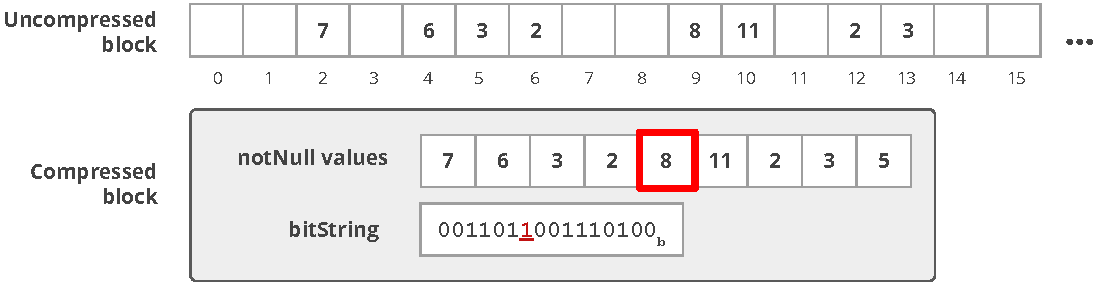
\includegraphics[scale=0.70]{img/null1}\hspace*{\fill}
	\captionsetup{justification=centering}
	\caption{\texttt{NULL} compression using bit-Strings.}
	\label{fig:null1}
	\vspace{-5pt}
\end{figure}

A more generalized \texttt{NULL} compression technique is based on using bit-string to indicate if the location is empty or not. In particular, we assign a \texttt{NULL} bit for each element in the column to indicate if the value at that location is a \texttt{NULL} or not. Figure \ref{fig:null1} shows the \texttt{NULL} enocding of an uncompressed column using this scheme. The column is divided into block, where each compressed block holds 2 pieces of information: 1) a \textbf{non-NULL values array} that holds the values in the block of uncompressed column that are not \texttt{NULL}, and 2) a \textbf{bit-string} having a bit for each element, with 1's at non NULL locations. Hence, the storage overhead is only that of a bit-string which is 1 bit per element in the uncompressed column or 0.5 bit per non NULL element for a column that is 50\% occupied. Based on the sparsity, bit-string can be replaced by a list of offsets of non \texttt{NULL} locations for very sparse data, or list or ranges of non \texttt{NULL} values for very dense data.

The above described compression scheme is not applicable to our scenario. Even though it is possible to operate on compressed column, the proposed scheme do not cater to our requirement of constant time random access. Reading from a location involves iterating over the bit-string to calculate the index of the element in the non-\texttt{NULL} values array. For instance, in fig~\ref{fig:null1}, accessing the element at index 9 involves counting the number of 1's till before index 9, which is 4. Thus, the value is read from index 5 of the non-\texttt{NULL} values array.

\section{PrefixSum-based NULL Compression}
\label{sec:prefixbased}

We present the solution to overcome the problem of constant time random reads in the existing solutions for compressing \texttt{NULL}s in sparse columns. The high-level idea is to do away with iteration over the bit-string while accessing the particular element in the compressed column.

\begin{figure}
	\vspace{-20pt}
	\hfill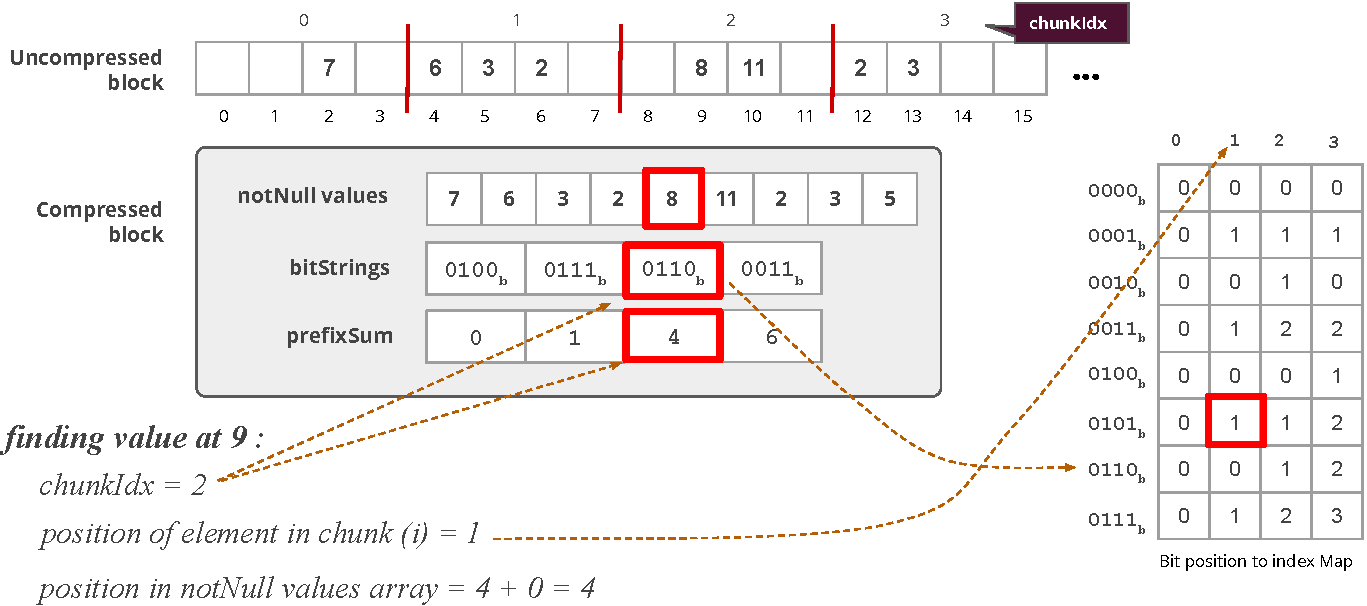
\includegraphics[scale=0.70]{img/null2}\hspace*{\fill}
	\captionsetup{justification=centering}
	\caption{PrefixSum-based \texttt{NULL} compression scheme. Chunk Size (n) = 4}
	\label{fig:null2}
	\vspace{-2pt}
\end{figure}

Figure~\ref{fig:null2} depicts compression of an uncompressed sparse column using our scheme, which we call \emph{prefixSum-based NULL compression}. It divides the column into chunks of fixed size $n$. A compressed block contains 3 peices of information: 1) a non-\texttt{NULL} values array, 2) a bit-string per chunk with 1's at not \texttt{NULL} locations in the chunk, and 3) prefixSum per chunk which is the cummulative count of non \texttt{NULL} in previous chunks. We also maintain a pre-populated 2D map in the memory having size $(2^n, n)$. We call this \emph{bit position to index map}. Given a valid bit-string $b$ of length $n$ and a position in the bit-string $i$, the map returns the number of 1's that appear in the bit-string before the queried position. The purpose of this map is to return the number of 1's that appear before the position $i$ in $b$. Using the map, we can avoid iteration over the bit-string to get the index of the element at position $i$ in the non-\texttt{NULL} values array, in the chunk.



















